\section{Compare the results of the second user journey}\label{section:results:comparison-second-journey}

This section compares the results for a second user journey through the prototype between the three approaches explained in Section \ref{section:results:performance-measurement}. The client's journey through the application is shown in Figure \ref{fig:results:evaluation-second-path}. The client has to perform 17 steps throughout the prototype, which involves running every available GraphQL query. In contrast to the first journey from Section \ref{section:results:comparison-first-journey}, the client uses an authenticated user to perform the test. The GraphQL \ac{API} query to retrieve the authenticated user is performed by every micro-frontend individually.

\ifshowImages
\begin{figure}[H]
  \centering
  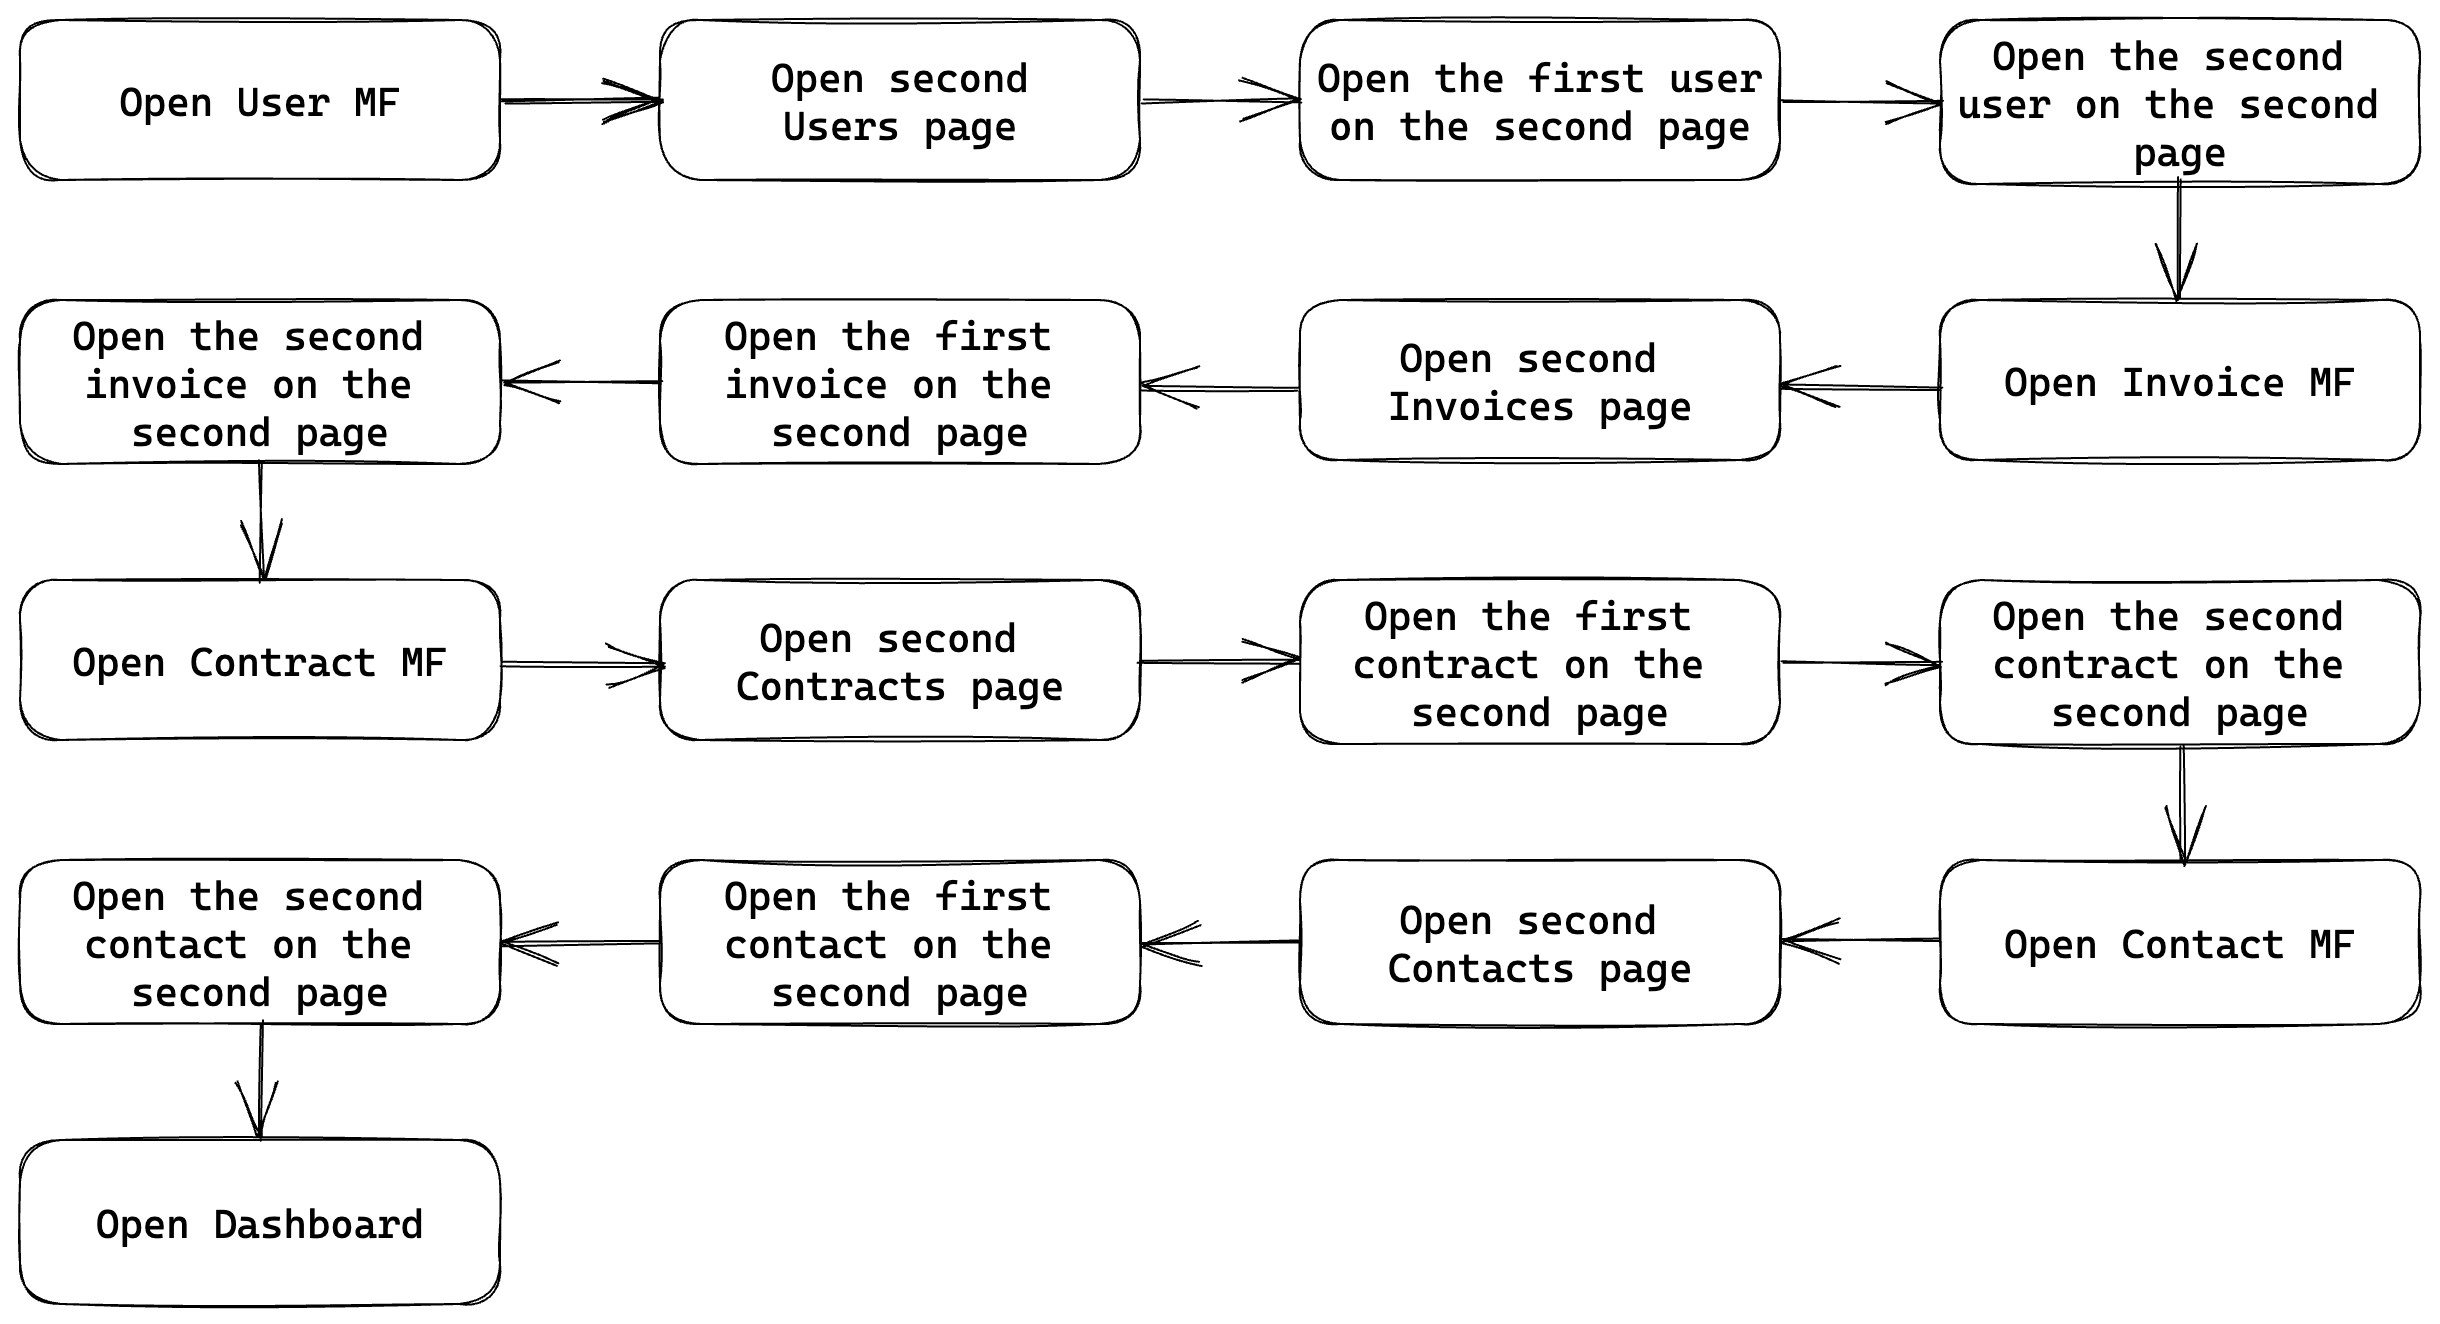
\includegraphics[width=1\linewidth]{images/results/evaluation-second-path.png}
  \caption{The second user journey through the application to measure the performance of the micro-frontend architecture.}\label{fig:results:evaluation-second-path}
\end{figure}
\fi

\noindent The following sections compare the three distinct approaches regarding request size, response size, number of requests, and the total number of records fetched, just as in the previous Section \ref{section:results:comparison-first-journey}.

\subsection{Compare the first- and second-approach}\label{subsection:results:comparison-second-path-first-second-approach}

Comparing the first approach with the second, there is a difference of 25 network requests to the GraphQL \ac{API} and the size of the requests and responses, as seen in Table \ref{table:results:size-comparison-second-path-cache-no-reduction-cache-reduction}. The second approach requires 25 fewer network requests than the first approach. Since the queries are not altered for this comparison, the additional network requests are responsible for the overall difference in request- and response size. The difference in request size is 26\%, which is about 6.07 KB, which is insignificant. Using a shared cache layer can save about 22\% of the total response size. Another interesting observation is that the shared cache approach retrieves 30401 fewer records than the naive approach, which is about 37\% of the total records returned.

\ifshowTables
\begin{table}[H]
  \begin{tabular}{|l|l|l|l|l|}
  \hline
  & \textbf{Req. size (B)} & \textbf{Resp. size (B)} & \textbf{Requests} & \textbf{Records} \\
  \hline
  \textbf{No Reduction, Separate Cache} & 22955 & 10713304 & 62 & 81325 \\
  \hline
  \textbf{No Reduction, Shared Cache} & 16884 & 8364416 & 37 & 50924 \\
  \hline
  \hline
  \textbf{Diff (B)} & \textbf{6071} & \textbf{2348888} & \textbf{25} & \textbf{30401} \\
  \hline
  \textbf{Reduction (\%)} & \textbf{26\%} & \textbf{22\%} & \textbf{40\%} & \textbf{37\%} \\
  \hline
  \end{tabular}
  \caption{Second Journey: Compare the requests and responses of the second- and third-approach.}\label{table:results:size-comparison-second-path-cache-no-reduction-cache-reduction}
\end{table}
\fi

\subsection{Compare the first- and third-approach}\label{subsection:results:comparison-second-path-second-third-approach}

As in the previous comparison, there are again 25 requests less made to the GraphQL \ac{API}. The size of the responses and the requests are similar to the previous section. The results are shown in Table \ref{table:results:size-comparison-second-path-no-cache-no-reduction-cache-reduction}. However, due to the reduction in queries, the difference in the size of queries and responses is more pronounced than in Section \ref{subsection:results:comparison-second-path-first-second-approach}. The difference in request size is 36\%, which accounts for 8.24 KB, which is insignificant. A shared caching layer and query reduction can save about 22\% of response size; as before, 37\% fewer records need to be fetched from the GraphQL \ac{API}.

\ifshowTables
\begin{table}[H]
  \begin{tabular}{|l|l|l|l|l|}
  \hline
  & \textbf{Req. size (B)} & \textbf{Resp. size (B)} & \textbf{Requests} & \textbf{Records} \\
  \hline
  \textbf{No Reduction, Separate Cache} & 22955 & 10713304 & 62 & 81325 \\
  \hline
  \textbf{Reduction, Shared Cache} & 14718 & 8361306 & 37 & 50924 \\
  \hline
  \hline
  \textbf{Diff (B)} & \textbf{8237} & \textbf{2351998} & \textbf{25} & \textbf{30401} \\
  \hline
  \textbf{Reduction (\%)} & \textbf{36\%} & \textbf{22\%} & \textbf{40\%} & \textbf{37\%} \\
  \hline
  \end{tabular}
  \caption{Second Journey: Compare the requests and responses of the first- and third-approach.}\label{table:results:size-comparison-second-path-no-cache-no-reduction-cache-reduction}
\end{table}
\fi

\subsection{Compare the second- and third-approach}\label{subsection:results:comparison-second-path-first-third-approach}

Between the second and third approach, there is almost no difference regarding request size and response size. The results are displayed in Table \ref{table:results:size-comparison-second-path-no-cache-no-reduction-cache-no-reduction}. Both approaches have the same number of queries sent to the GraphQL \ac{API} and receive the same number of records since all micro-frontends share the same cache instance. The difference in request and response size comes solely from using the query reduction mechanism. The difference in request size is 13\%, but they account for just 2.17 KB, which is insignificant. The difference between the response sizes (3.11 KB) is almost zero, like in the first user journey.

\ifshowTables
\begin{table}[H]
  \begin{tabular}{|l|l|l|l|l|}
  \hline
  & \textbf{Req. size (B)} & \textbf{Resp. size (B)} & \textbf{Requests} & \textbf{Records} \\
  \hline
  \textbf{No Reduction, Shared Cache} & 16884 & 8364416 & 37 & 50924 \\
  \hline
  \textbf{Reduction, Shared Cache} & 14718 & 8361306 & 37 & 50924 \\
  \hline
  \hline
  \textbf{Diff (B)} & \textbf{2166} & \textbf{3110} & \textbf{0} & \textbf{0} \\
  \hline
  \textbf{Reduction (\%)} & \textbf{13\%} & \textbf{0\%} & \textbf{-} & \textbf{-} \\
  \hline
  \end{tabular}
  \caption{Second Journey: Compare the requests and responses of the first- and second-approach.}\label{table:results:size-comparison-second-path-no-cache-no-reduction-cache-no-reduction}
\end{table}
\fi